\documentclass{report}

\usepackage{polski} % Pozwala na użycie polskiego. Ustawia między innymi fontenc na T1
\usepackage[utf8]{inputenc} % Informuje o kodowaniu

\usepackage{xcolor}% http://ctan.org/pkg/xcolor
\definecolor{LinkColor}{HTML}{1d5cc1} % Kolor do linków
\usepackage{hyperref}% http://ctan.org/pkg/hyperref

\definecolor{LinkColor}{HTML}{1d5cc1}

\usepackage{tabto}

\usepackage{graphicx} % Pakiet do obrazów
\graphicspath{ {./Obrazy/} } % Folder, z którego będą brane obrazy
\usepackage{float} % Dodatkowe pozycjonowanie obrazów - [H]
\usepackage{subcaption} % Kilka obrazów w jednej figurze

% Nie twórz nowych stron
\usepackage{etoolbox}
\makeatletter
% \patchcmd{\chapter}{\if@openright\cleardoublepage\else\clearpage\fi}{}{}{}
\makeatother

\title{Specyfikacja funkcjonalna -- Wireworld}
\author{Krzysztof Dąbrowski i Jakub Bogusz}
\date{\today}

\begin{document}
\maketitle{}

\tableofcontents{}

\chapter{Cel projektu}
Celem projektu jest implementacja automatu komórkowego Wire World w języku Java z interfejsem graficznym zaimplementowanym przy pomocy biblioteki JavaFX. Gotowy program ma pozwalać użytkownikowi przeprowadzać symulacje zgodne z określonymi zasadami. Parametrami generacji użytkownik będzie mógł sterować ręcznie przy pomocy graficznego \hyperref[sec:wyglad-gui]{\textcolor{LinkColor}{interfejsu użytkownika}}.

Interfejs będzie wyświetlał na bierząco podgląd kolejnych generacji. Użytkownik będzie miał możliwość wstrzymania symulacji oraz zmianę stanu planszy przy pomocy narzędzi edycji.

Ponadto będzie istnieć również możliwość przełączenia trybu symulacji z Wire World na automat komórkowy Game of life.

\chapter{Opis ogólny problemu}

\section{Wstęp}
Projektu skupia się na realizacji 3 głównych aspektów problemu. Są to odpowiednio automaty komórkowe ,,Game of Life'' i ,,Wireworld'' oraz wizualna prezentacja działania tych automatów. 

\section{Wire World}

Wire World jest automatem komórkowym wymyślonym przez Briana Silvermana w roku 1987.  Jest często używany do symulacji elementów elektronicznych operujących na wartościach bitowych. Pomimo prostoty reguł, jakie nim rządzą, za pomocą Wireworld można nawet stworzyć działający komputer.

\subsection{Symulacja}
\begin{minipage}{\textwidth} %Akapit ma być na jednej stronie
    \paragraph{Stany}  Komórka może znajdować się w jednym z czterech stanów:
    \begin{itemize}
    \item pusta,
    \item głowa elektronu,
    \item ogon elektronu,
    \item przewodnik.
    \end{itemize}
\end{minipage}

\paragraph{Pokolenie} to zbiór stanów wszystkich komórek w danej chwili. Gdy stan pokolenia jest ustalony, możliwe jest utworzenie nowego (potomnego) pokolenia komórek, powstających według poniższych zasad.

\paragraph{Reguły} Następne pokolenie generowane jest zgodnie z regułami:
\begin{itemize}
\item Jeżeli komórka jest pusta, to pozostaje pusta niezależnie od jej otoczenia,
\item Jeżeli komórka jest głową elektronu, to zmieni się w ogon elektronu,
\item Jeżeli komórka jest ogonem elektronu, to zmieni się w przewodnik,
\item Jeżeli komórka jest przewodnikiem i sąsiaduję z jedną lub dwoma komórkami będącymi głowami elektronu, to zmieni się w przewodnik.
\end{itemize}

\subsection{Struktury}
Symulacja przeprowadzona zgodnie z powyższymi regułami może prowadzić do powstania ciekawych obiektów zwanych strukturami. 
\begin{figure}[h]
\centering
\setlength{\fboxsep}{0pt} %Odstęp 0
\setlength{\fboxrule}{1pt} %Grubość ramki 1p
\fbox{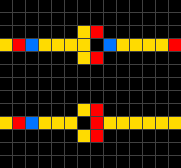
\includegraphics[width=8cm]{Obrazy/struktury_w.png}}
\caption{Przykłady struktur - dioda przewodząca i nieprzewodząca}
\end{figure}


\section{Game of life}

Game of life jest automatem komórkowym wymyślonym przez brytyjskiego matematyka John Horton Conway
w 1970 roku. Polega na symulacji kolejnych pokoleń życia komórek według następujących zasad.

\subsection{Symulacja}

\paragraph{Stany}  Komórka może znajdować się w jednym z dwóch stanów:
\begin{itemize}
\item żywa,
\item martwa.
\end{itemize}

\paragraph{Pokolenie} to stan wszystkich komórek w danej chwili. Gdy stan pokolenia jest ustalony, możliwe jest utworzenie nowego (potomnego) pokolenia komórek, powstających według poniższych zasad.

\paragraph{Reguły} Następne pokolenie generowane jest zgodnie z regułami:
\begin{itemize}
\item Jeżeli komórka była martwa i miała dokładnie 3 żywych sąsiadów, w następnym pokoleniu staje się żywa,
\item Jeżeli komórka była żywa to pozostaje żywa jeśli miała dwóch lub trzech żywych sąsiadów. W przeciwnym razie staje się martwa.
\end{itemize}

\subsection{Struktury}
Symulacja przeprowadzona zgodnie z powyższymi regułami może prowadzić do powstania ciekawych obiektów zwanych strukturami. 

\begin{figure}[h]
\centering
\setlength{\fboxsep}{0pt} %Odstęp 0
\setlength{\fboxrule}{1pt} %Grubość ramki 1p
\fbox{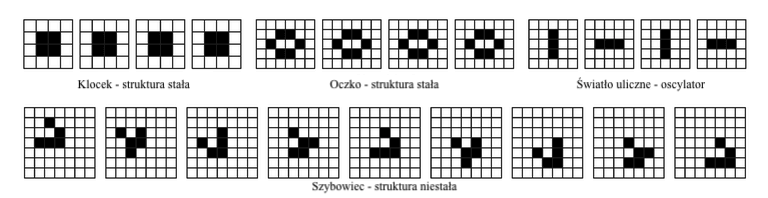
\includegraphics[width=13cm]{Obrazy/struktury.png}}
\caption{Przykłady struktur}
\end{figure}

Reguły symulacji umożliwiają również tworzenie dużo bardziej skomplikowanych struktur (jak na przykład maszyna Turinga -- https://youtu.be/My8AsV7bA94).

\section{Interfejs użytkownika}
\label{sec:opis-interfejs}
Ważnym aspektem programu jest sposób interakcji z użytkownikiem.
Realizowana aplikacja będzie obsługiwana poprzez graficzny interfejs użytkownika.

Interfejs pozwoli na poniższe funkcjonalności:
\begin{itemize}
    \item Bieżący podgląd stanu symulacji
    \item Możliwość dostosowania prędkości symulacji
    \item Zapis aktualnego pokolenia do pliku
    \item Wyczytanie pokolenia z pliku
    \item Edycje poszczególnych komórek w trakcie symulacji
    \item Wstawianie figur wybranch z przybornika
\end{itemize}

\chapter{Działanie programu}

\section{Opis komunikacji z użytkownikiem}
Po uruchomieniu programu zostanie wyświetlony graficzny interfejs, który pozwoli użytkownikowi sterować parametrami w dowolny sposób, zgodny z regułami symulacji. W razie wystąpienia błędów program będzie informować użytkownika wyświetlając nowe okno zawierające opis błędu.

W ramach interfejsu użytkownik będzie mógł wykonywać czynności opisane w punkcie \ref{sec:opis-interfejs} oraz przełączać między automatami Game of Life i Wireworld.

\section{Wygląd interfejsu użytkownika} \label{sec:wyglad-gui}
Interfejs użytkownika będzie wyglądał następująco. Wyszczególnione obszary są zaznaczone numerami.
\begin{figure}[H]
    \centering
    \includegraphics[width=0.99\columnwidth]{gui.png} %Dla 1 nie mieści się na tej samej stronie
    \caption{Całokształt interfejsu użytkownika}
\end{figure}

\section{Opis elementów}
\paragraph{1 Podgląd aktualnego stanu symulacji} \mbox{} \\
W tej części będzie wyświetlane bieżące pokolenie symulacji aktualnego automatu komórkowego. Po bokach panelu znajdują się \textbf{suwak} pozwalające na zminę oglądanego obszaru planszy. Będą one szczególnie przydatne po przybliżeniu obrazu.

\paragraph{2 Ustawienia symulacji i planszy} \mbox{} \\
Sekcja kontrolek umożliwiających sterowanie symulacją oraz zminę całości planszy.

Po lewej stronie znajduje się grupa elementów wpływających bezpośrednio na podgląd symulacji.
\begin{itemize}
    \item Play -- uruchamia automatycznie przechodzenie między staniami symulacji,
    \item Stop -- zatrzymuje automatycznie przechodzenie między staniami symulacji,
    \item Speed -- zmienia tempo automatycznego przechodzenie między staniami symulacji,
    \item Next generation -- ręczne przejście do następnego stanu symulacji,
    \item Zoom -- zmienia skalę podglądu aktualnego stanu.
\end{itemize}

Po prawej stronie umieszczona jest grupa elementów pozwalających na reset całego stanu planszy.
\begin{itemize}
    \item Grid height, Grid height -- wprowadzenie rozmiaru planszy jaka zostanie utworzona,
    \item Create -- Tworzy plansze o podanym rozmiarze, gdy plansza już istnieje i podany rozmiar jest równy planszy już istniejącej, opis 			przycisku zamienia się na "Clear", i wciśnięcie go zmienia stan wszystkich komórek na "Pusty" w przypadku WireWorld lub "Martwy" w 		przypadku Game of Life,
    \item Random -- Nadanie wszystkim komórkom losowych stanów,
\end{itemize}
%TODO: Przemyśleć co robią guziki Crate i Random. Ewentualnie przenieść tu guzik do wczytywania z planszy.

\paragraph{3 Przybornik} \mbox{} \\
Boczny przybornik zawierał będzie dwie zakładki, które będą pozwalały na edycje fragmentów planszy.

\begin{figure}[H]
    \centering
    \begin{subfigure}[b]{0.49\textwidth}
        \centering
        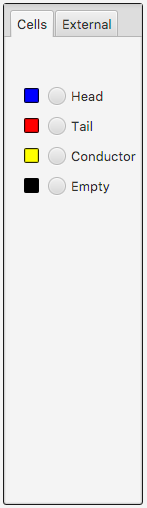
\includegraphics[width=0.4\textwidth]{przybornik1}
        \caption{Przybornik Cells}
    \end{subfigure}
    \begin{subfigure}[b]{0.49\textwidth}
        \centering
        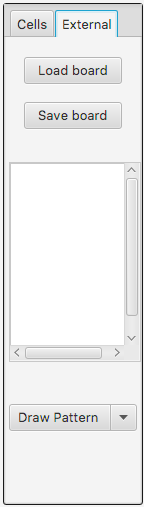
\includegraphics[width=0.4\textwidth]{przybornik2}
        \caption{Przybornik External}
    \end{subfigure}
\end{figure}

Zakładka \textbf{Cells} umożliwi wybranie stanu komórki, a następnie nadanie komórkom wybranego stanu poprzez klikanie myszą komórek w oknie podglądu.

Zakładka \textbf{External} da dostęp do zestawu gotowych figur, które użytkownik będzie mógł wstawić w wybranym miejscu planszy. Użytkownik będzie mógł dodać własne figury do przybornika oraz zapisać i wczytać stan całej planszy przy pomocy guzików z tej zakładki.

\paragraph{4 Wybór automatu} \mbox{} \\
Wstążka pozwalająca na zmianę aktywnego automatu komórkowego.

\section{Stany interfejsu}
Podczas korzystania z aplikacji interfejs będzie ulegał drobnym zmianom. Głównie elementy odpowiadające za aktualnie niedostępne opcje będą zmieniać kolor na szary.

\subsection{Po włączeniu programu}
Większość kontrolek jest \textbf{wyłączonych} do momentu wczytania planszy z pliku lub wygenerowania losowej. Program domyślnie wyświetla okno symulacji automatu Wireworld.

\begin{figure}[H]
    \centering
    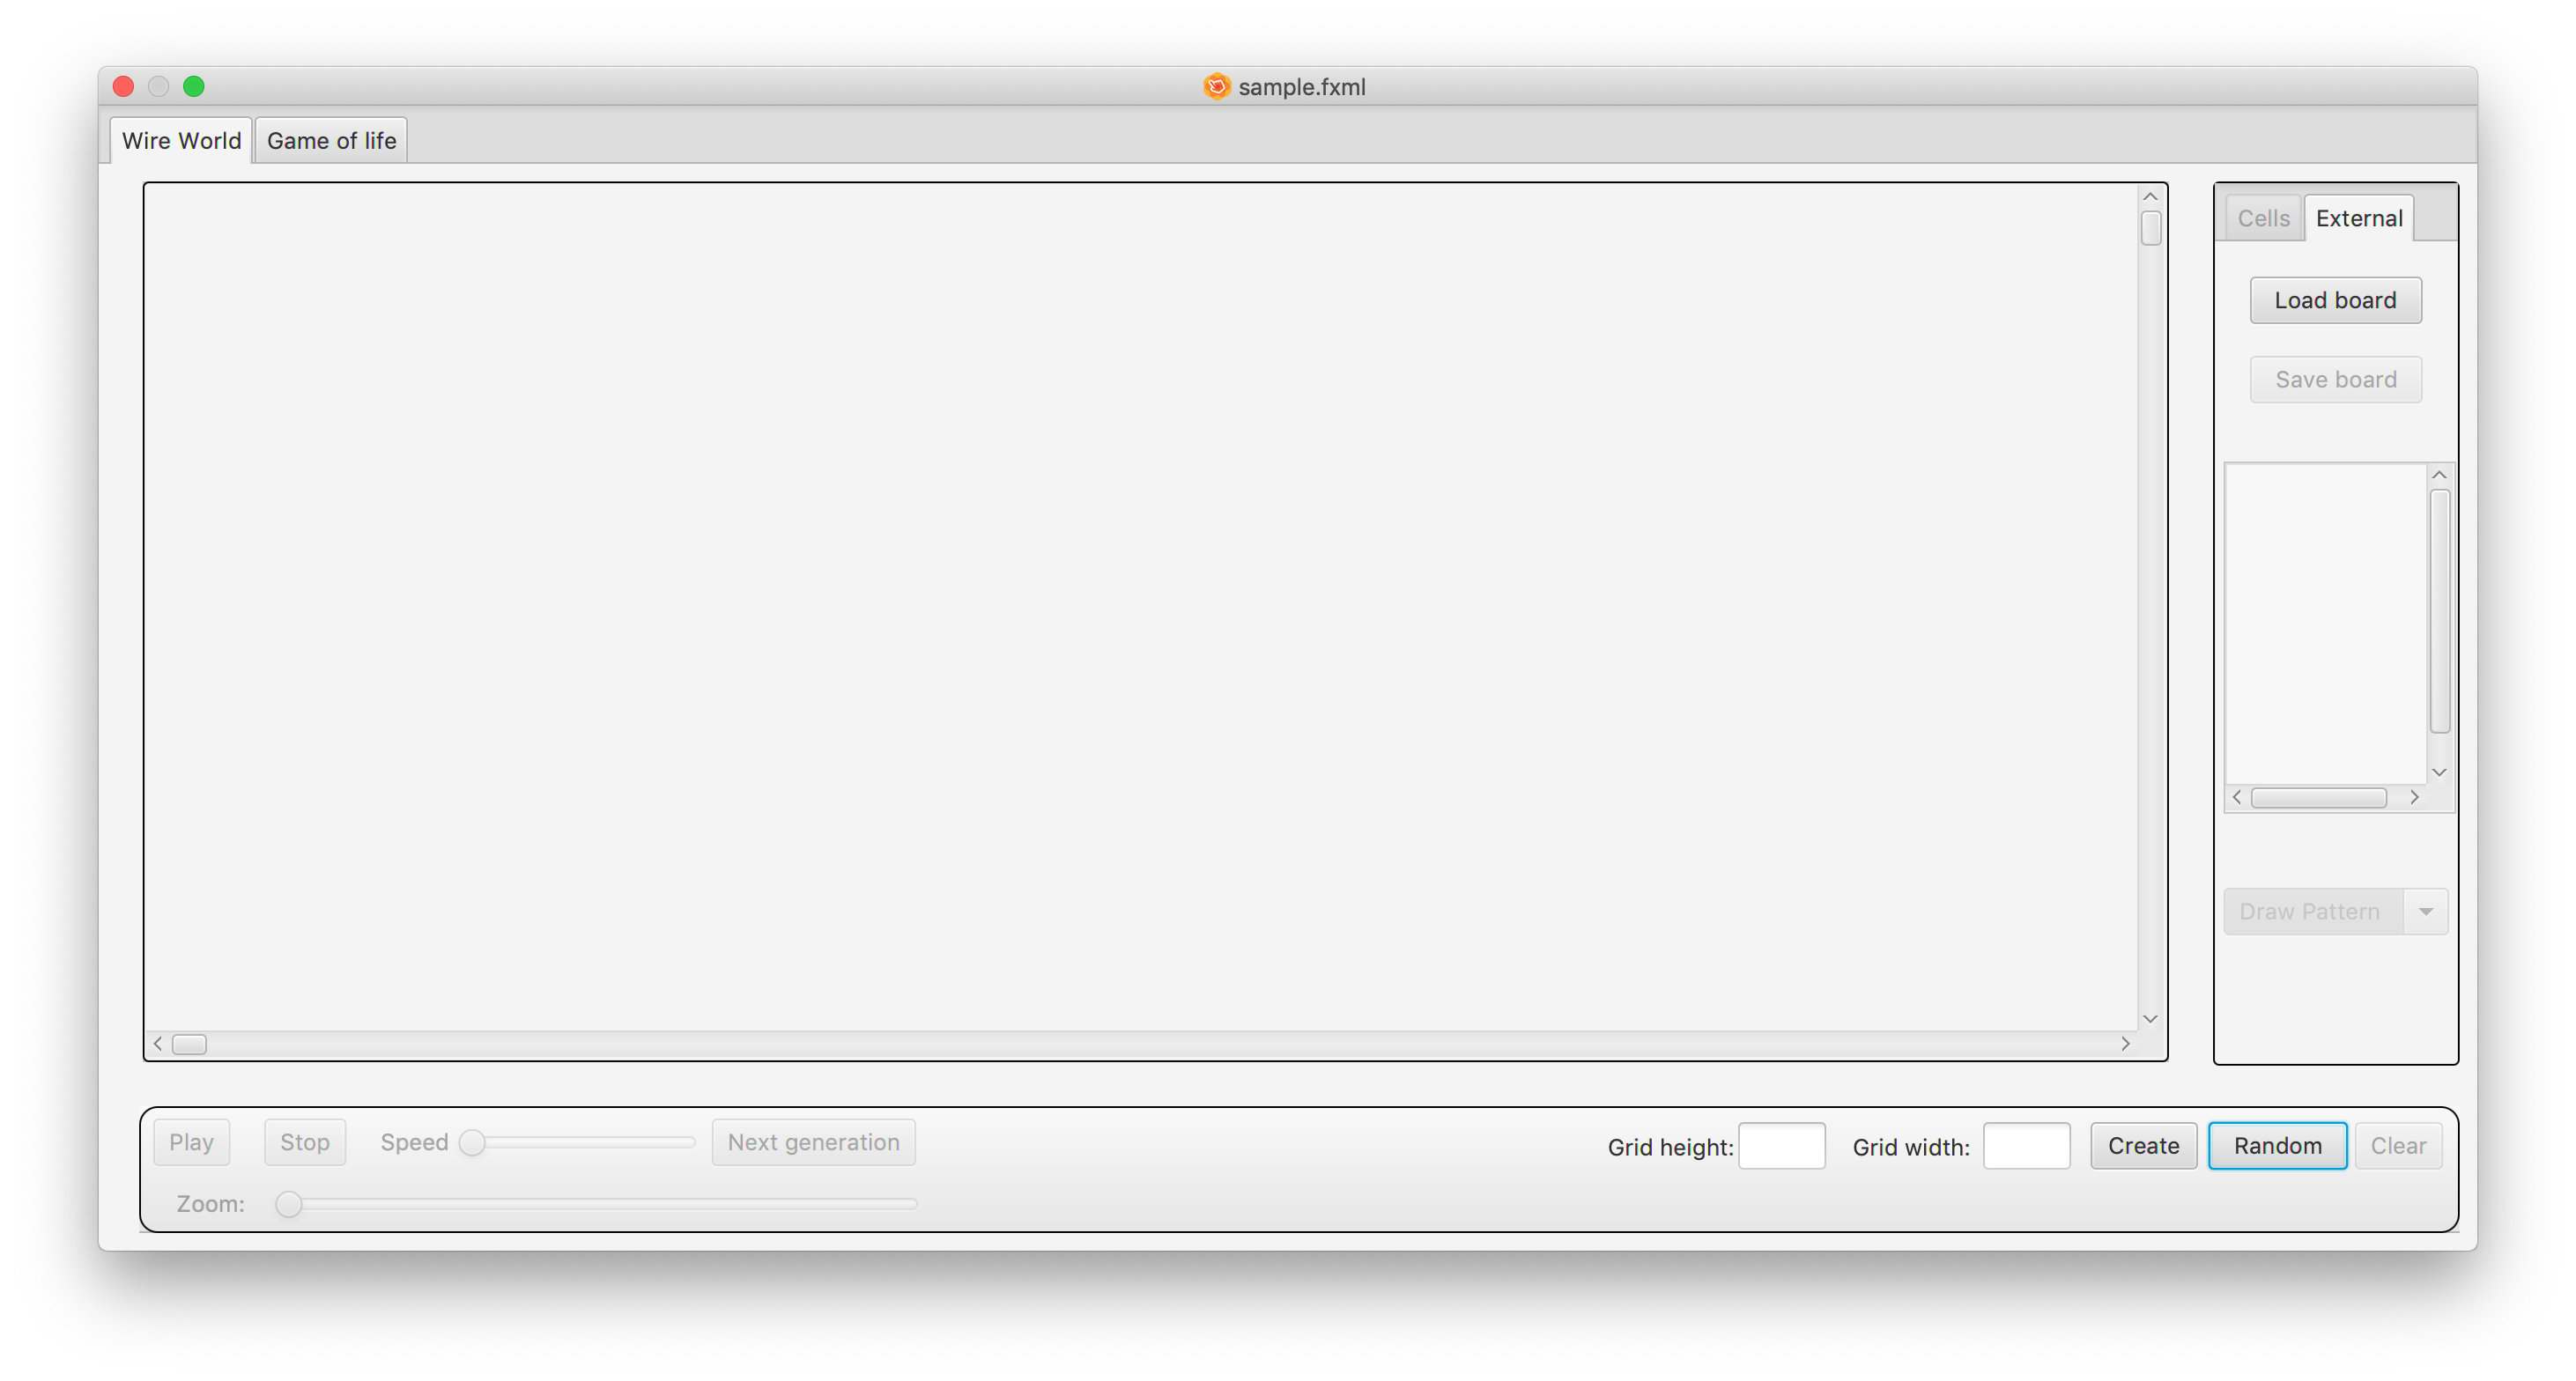
\includegraphics[width=\textwidth]{gui-initial}
    \caption{Stan interfejsu po uruchomieniu aplikacji}
\end{figure}

\subsection{W trakcie symulacji}
Można zmienić tempo symulacji oraz wstrzymać generację następnych pokoleń, co umożliwi edycję aktualnego pokolenia.

\begin{figure}[H]
    \centering
    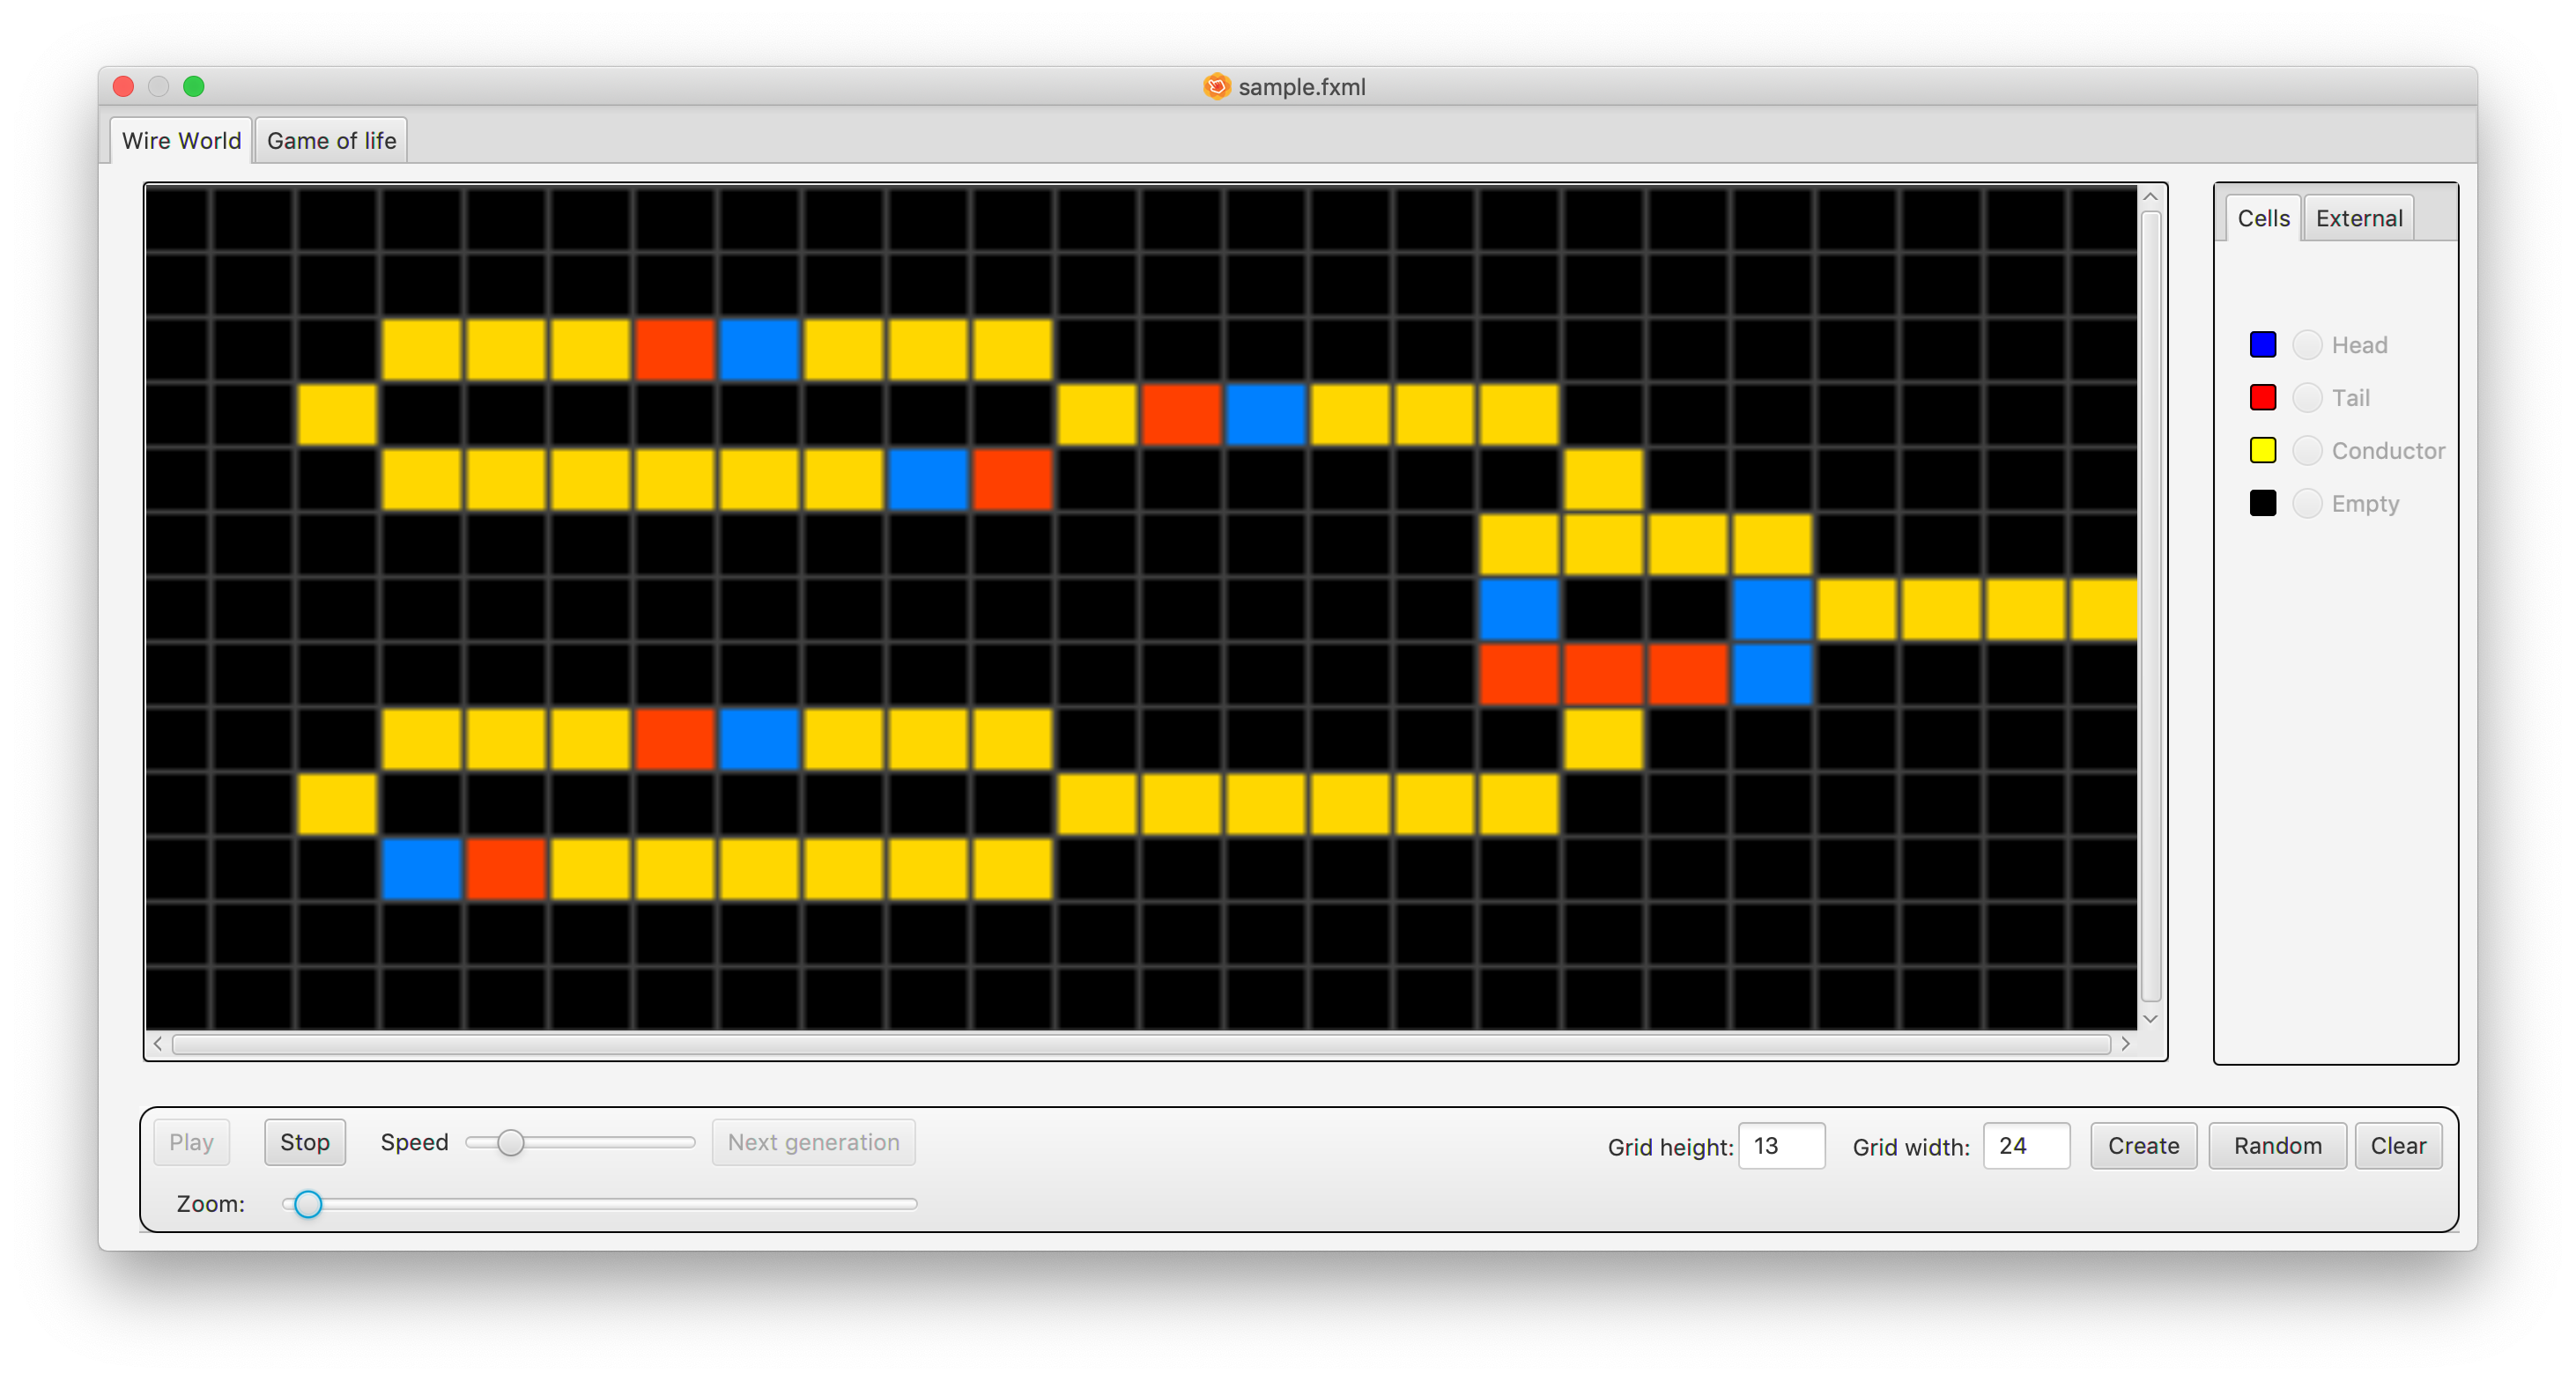
\includegraphics[width=\textwidth]{gui-running}
    \caption{Stan interfejsu w trakcie symulacji}
\end{figure}

\subsection{Symulacja wstrzymana}
Możliwe jest edytowanie komórek przy pomocy narzędzie oraz wstawianie figur.

\begin{figure}[H]
    \centering
    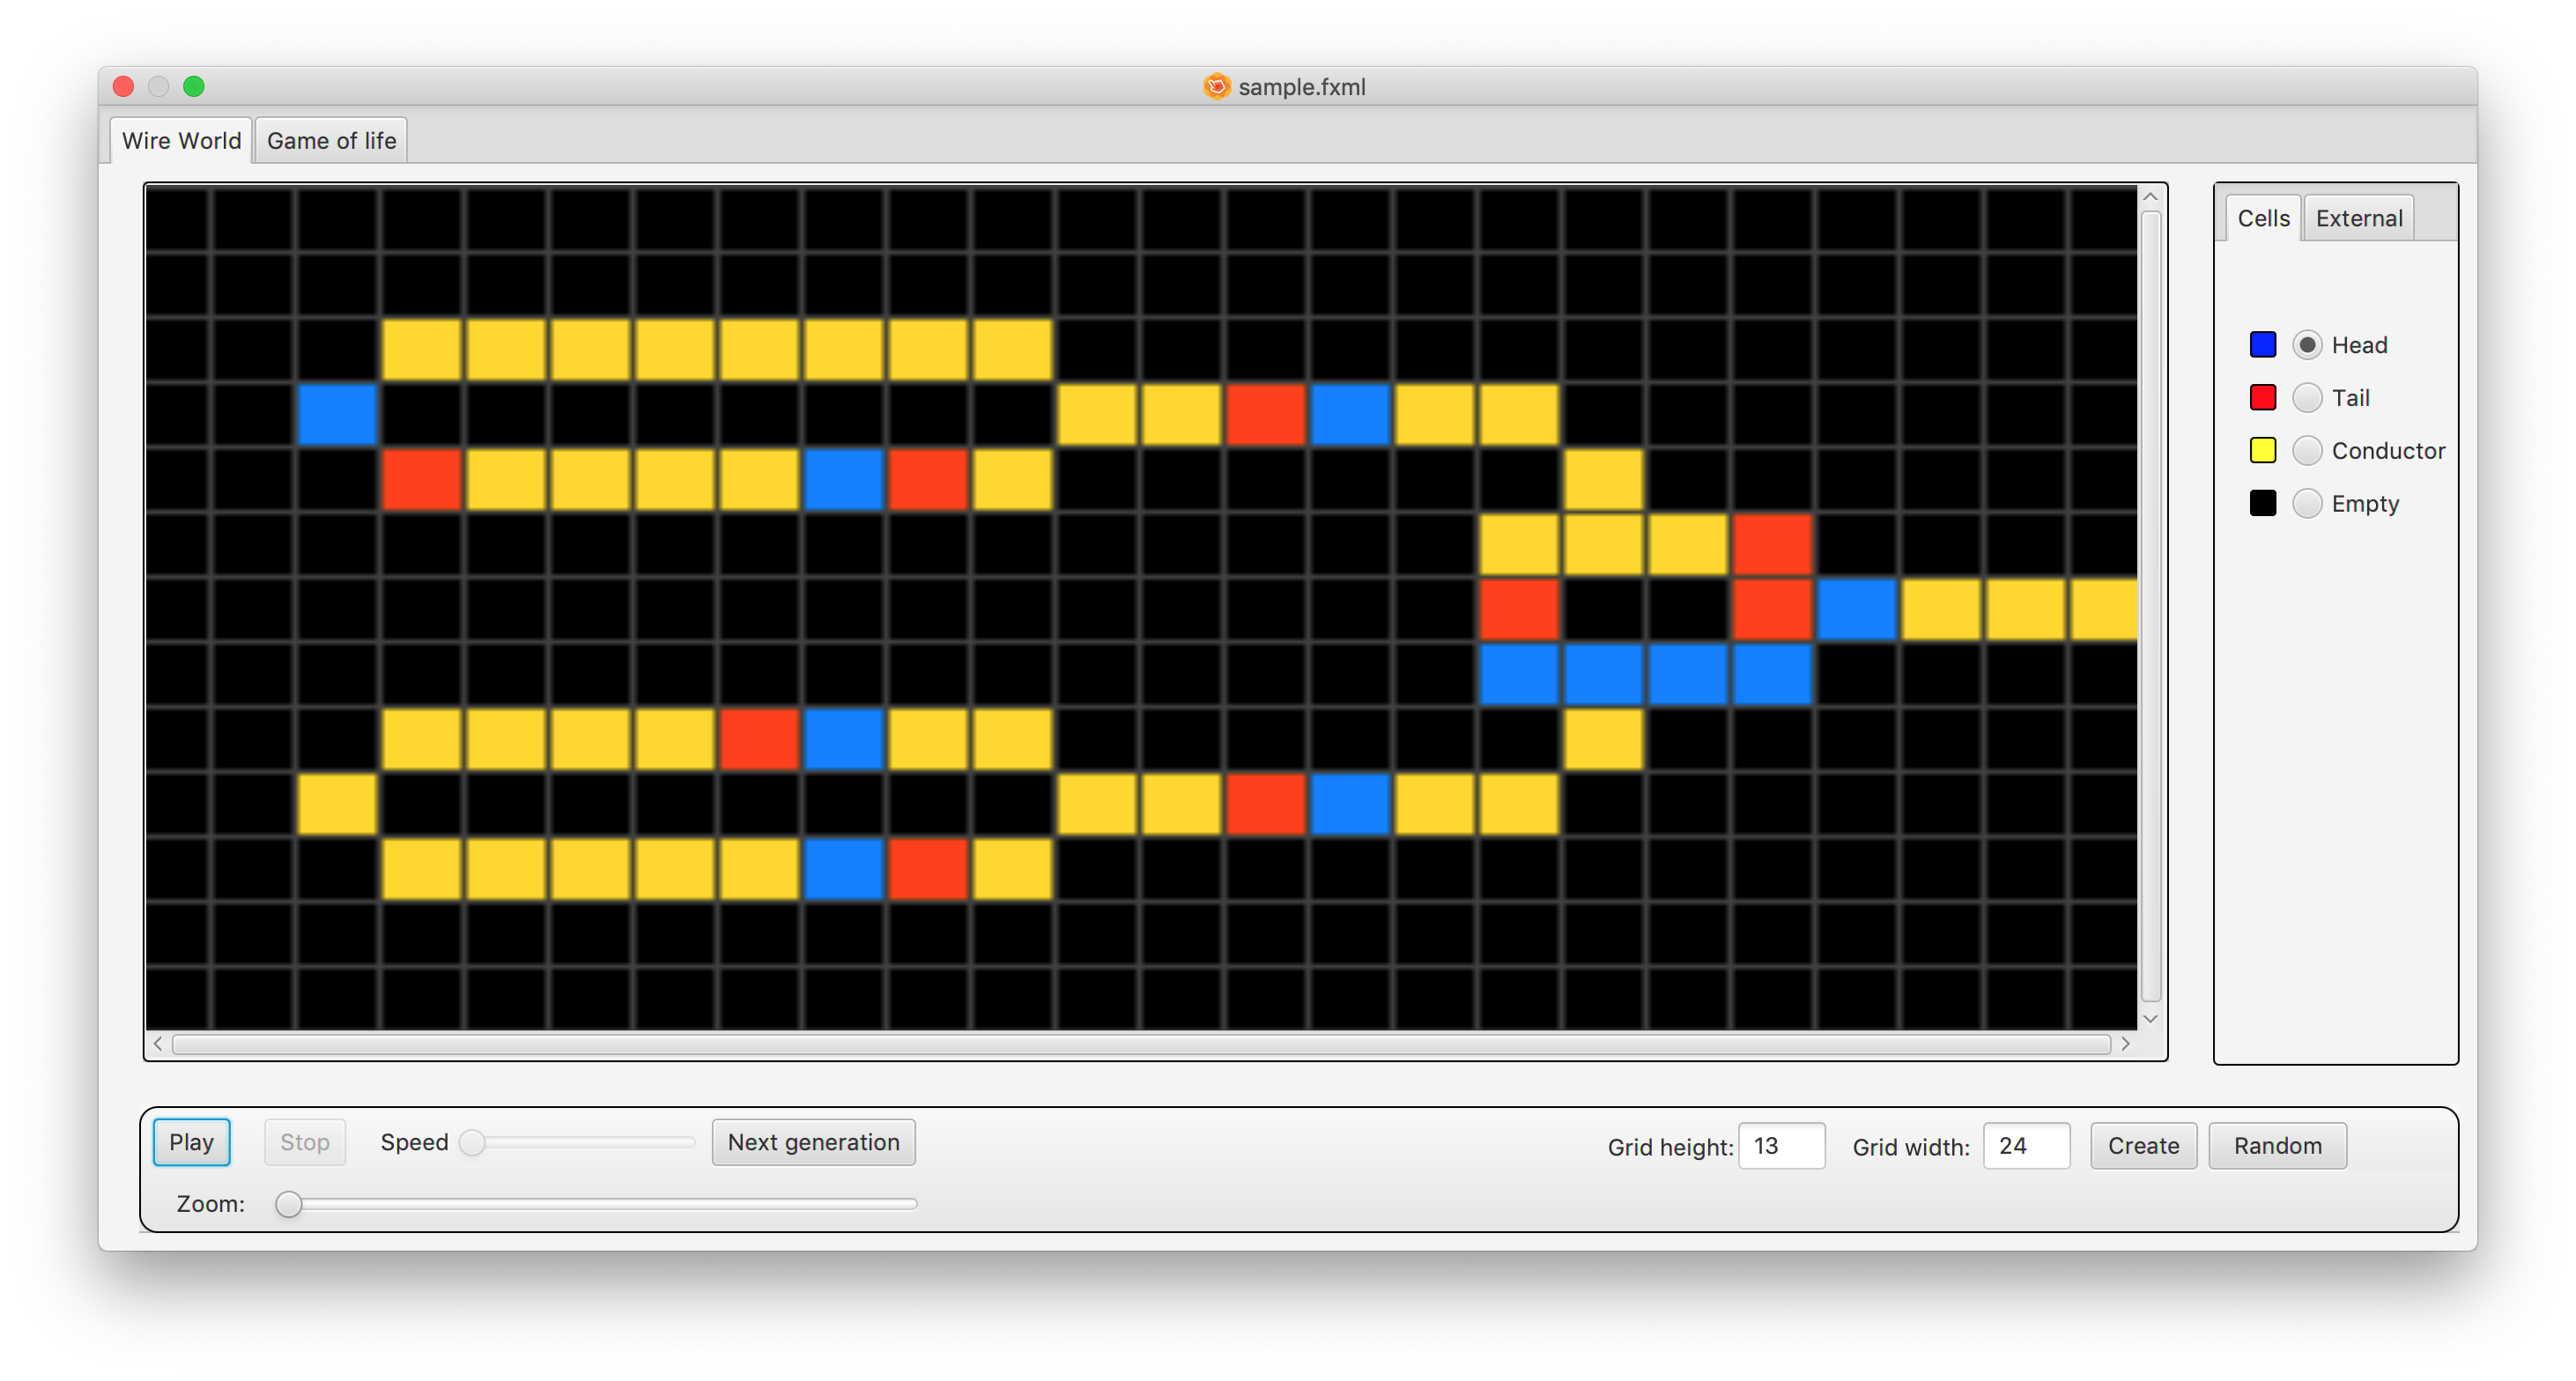
\includegraphics[width=\textwidth]{gui-paused}
    \caption{Stan interfejsu przy wstrzymanej symulacji}
\end{figure}

\section{Tryb automatu Game of Live}
Program obsługuje również automat komórkowy Game of Live. Przełączenie między aktualnym automatem jest realizowane przy pomocy wstążki na górze interfejsu.
Większość elementów interfejsu pozostanie taka sama jak w automacie Wireworld. Inaczej będzie wyglądał przybornik do edycji planszy, ponieważ automat ten zawiera inne stany komórek.

%TODO: Usunąć lub wykorzystać ten komentarz
%\begin{figure}[h]
%\centering
%\setlength{\fboxsep}{0pt} %Odstęp 0
%\setlength{\fboxrule}{1pt} %Grubość ramki 1p
%\fbox{\includegraphics[width=13cm]{Obrazy/gui.png}}
%\caption{Przykłady struktur}
%\end{figure}

\chapter{Edycja planszy}
Użytkownik ma kilka możliwości na wgranie planszy do programu lub edycję już istniejącej. Są one wymienione poniżej.

\section{Plik wejściowy}  \label{format}
Program pozwala na wczytanie całego stanu planszy (wraz z rozmiarem) z pliku. Dzięki temu możliwe jest łatwe odtworzenie stanu ze wcześniejszej symulacji lub prezentacja skomplikowanego układu.

Program będzie w stanie obsłużyć różnie formaty plików wymienione poniżej.

\subsection{JSON}
W celu nadania danym przenośności, oraz ułatwienia generacji danych przy pomocy zewnętrznych narzędzi zostanie wykorzystany format JSON. Jest to \textbf{domyślny format} zapisu planszy.

\subsubsection{Przykład}
Przykład zapisu przedstawionej planszy. 

\begin{figure}[H]
    \centering
    
\includegraphics[height=4cm]{przyklad-planszy-wireworld}
    \caption{Przykładowa plansza}
\end{figure}

\noindent{}Plik reprezentujący planszę:
\begin{verbatim}
{
  "width" : 2,
  "height" : 3,
  "states" : [ "HEAD", "TAIL", "HEAD", "HEAD", "HEAD", "EMPTY" ]
}
\end{verbatim}

\subsection{XML}
Możliwy jest również zapis stanu planszy do pliku XML. Z uwagi na mniejszą czytelność oraz większy rozmiar plików tego typu nie jest to domyślnie używany format. Użytkownik będzie miał możliwość zmiany formatu pliku, do jakiego chce zapisać planszę przy pomocy interfejsu graficznego.

\subsubsection{Przykład}
Przykład zapisu przedstawionej planszy. 

\begin{figure}[H]
    \centering
    
\includegraphics[height=4cm]{przyklad-planszy-wireworld}
    \caption{Przykładowa plansza}
\end{figure}

\begin{samepage}
\noindent{}Plik reprezentujący planszę:
\begin{verbatim}
<Board>
  <width>2</width>
  <height>3</height>
  <states>
    <states>CONDUCTOR</states>
    <states>HEAD</states>
    <states>TAIL</states>
    <states>TAIL</states>
    <states>CONDUCTOR</states>
    <states>EMPTY</states>
  </states>
</Board>
\end{verbatim}
\end{samepage}


\section{Przybornik stanów}
Jedną z części interfejsu użytkownika będzie przybornik pozwalający na wybór jednego ze stanów aktualnego automatu komórkowego. Po zaznaczeniu jednego ze stanów użytkownik będzie miał możliwość zamiany wybranych komórek aktualnego pokolenia na wybrany stan.

\section{Wstawianie figur}
Interfejs będzie zawierał zestaw typowych figur dla aktualnego automatu komórkowego. Możliwe będzie zaznaczenie wybranej figury oraz wstawienie jej w wybrane miejsce symulacji.

\subsection{Rozszerzanie listy figur}
%TODO: Przemyśleć Rozszerzanie listy figur do wklejenia i ich zapisywanie
Użytkownik będzie miał możliwość dodania własnych figur do domyślnej listy.

\section{Zapis stanu planszy}
Program będzie w stanie zapisać aktualny stan planszy w formacie, który umożliwi późniejsze  wczytanie planszy.
%TODO: Czy użytkownik będzie mógł wybrać format?

\chapter{Sytuacje wyjątkowe}
%TODO Sytuacje wyjątkowe
Czasem działanie programu może ulec zmianie na skutek nieprawidłowych danych wejściowych, niestandardowych ustawień wprowadzonych przez użytkownik lub z przyczyn losowych. Ten rozdział opisuje jak program zachowa się w takiej sytuacji, oraz co może ją wywołać.

\section{Zmiana domyślnego zachowania}
\paragraph{Zbyt szeroka plansza}
W przypadku gdy użytkownik włączy wyświetlanie kolejnych stanów w konsoli ale rozmiar planszy będzie zbyt szeroki by możliwe było jej wyświetlenie bez zawijania wierszy program wyświetli komunikat o niemożliwości wyświetlenia planszy w konsoli. Kolejne pokolenia nie będą wyświetlanie oknie wiersza poleceń ale generacja plików wynikowych nie ulegnie zmianie. \\
Treść komunikatu: ,,Wybrana szerokość planszy jest zbyt duża by możliwe było wyświetlenie kolejnych pokoleń w oknie konsoli.''

\section{Błędy}
Opis błędów, które mogą wystąpić w trakcie działania programu.

\subsection{Błędy pliku wejściowego}

\paragraph{Podany plik nie istnieje}
Jeśli ścieżka podana przez użytkownika jest błędna program wyświetli komunikat o braku możliwości otwarcia wskazanego pliku i zakończy pracę. \\
Treść komunikatu: ,,Nie udało się otworzyć wskazanego pliku.''

\paragraph{Pusty plik}
W przypadku gdy plik wskazany przez użytkownika będzie pusty program powiadomi o tym i zakończy pracę. \\
Treść komunikatu: ,,Wskazany plik wejściowy jest pusty.''

\paragraph{Rozmiar planszy nie będący liczbą}
Jeśli w pierwszej lini pliku znajdować się będą wartości inne niż liczby program nie będzie w stanie wczytać rozmiaru planszy. W takiej sytuacji wyświetli odpowiedni komunikat i zakończy pracę. \\
 Treść komunikatu: ,,Nie udało się wczytać rozmiaru planszy.''
 
 \paragraph{Niedodatni rozmiar planszy}
 Jeśli jeden z wymiarów planszy nie będzie dodatnią liczbą całkowitą program zasygnalizuje błąd i zakończy pracę. \\
 Przykładowy komunikat: ,,Szerokość musi być większa od 0. Podana szerokość to -5.''
 
 \paragraph{Brak nowej linii po rozmiarze planszy}
 W przypadku gdy po wysokości planszy w pliku będzie inny znak niż przejście do nowej lini program zasygnalizuje błąd i zakończy pracę. \\
 Treść komunikatu: ,,Spodziewany koniec lini po wymiarze planszy.''
 
 \paragraph{Błąd przy wczytywaniu stanu komórki}
 Jeśli nie uda się wczytać stanu komórki, na przykład ponieważ w pliku jest za mało linii lub jedna z linii jest zbyt krótka, program wypisze, w którym miejscu pliku wystąpił błąd i zakończy pracę. \\
 Przykładowy komunikat: ,,Wystąpił błąd przy próbie przeczytania znaku w lini: 3 kolumnie: 8.''
 
 \paragraph{Nieprawidłowy znak w pliku}
 Jeśli podczas czytania pliku program napotka nieprawidłowy znak wypisze na jakiej pozycji w pliku napotkany został nieprawidłowy znak, jaki to znak, oraz czego spodziewał się program. \\
 Przykładowy komunikat: ,,Niewspierany znak napotkany w lini: 2 kolumnie: 1. Spodziewana wartość: 0 lub 1. Napotkana wartość: T''

\subsection{Błędy losowe}
\paragraph{Brak pamięci operacyjnej}
Gdyby w systemie zabrakło pamięci program nie będzie w stanie funkcjonować poprawnie. Program wyświetli komunikat o błędzie i przerwie pracę. \\
Treść komunikatu: ,,Program nie uzyskał pamięci od systemu operacyjnego. Spróbuj uruchomić program ponownie za pewien czas.''

\end{document}
